\chapter{About Clustering, Correlation and Expression}
\label{ch:expression}

\setlength{\epigraphwidth}{0.45\textwidth}
\setlength{\epigraphrule}{0.1pt}
\epigraph{Quantifier: c'est convenir, puis mesurer.}{\cite{Desrosieres}}

\section{Introduction}

As a former chemist, I realise how much it is tempting to trust instruments and
workflow to accurately identify and quantify all the molecules present in a sample,
and then been confounded\footnote{After more than 4 months of identification attempts
with various modern techniques, what could have been the orange/red spot
(visible light) at 1/3 of that tight light chromatogram is still a mystery too me.}.
Hence, I tried to avoid as much as I could any source of technical
artefacts and biases in the data and statistical approaches I used for these
exploratory analyses.

As we know the tissue type for each sample of each dataset,
we could debate that supervised analyses can be more informative.
However, they would involve proper corrections
for batch effects and other technical biases for each dataset.

This is challenging as that often requires more knowledge than the available one
through the repositories. It is also unwise to rely solely on the normalised data
provided by the original authors as bias corrections (when possible)
in \Rnaseq\ will vary in function of the following downstream analyses.
Likewise, proteomic data is hard to handle and from the same data,
two identification/quantification pipelines can give rather quite
different results (see~\Cref{ch:proteomics}).

To assess the consistency, in particular for \Rnaseq, quantification across
the different datasets, I chose a widely used and unsupervised method for gene
expression studies: a clustering analysis.

\section{Clustering analysis}

This method uncovers possible hidden structures within the data, therefore,
it is well designed for exploratory studies.
I can thus confirm if samples are more alike either due to their
biological or their study origins. In general, we expect biology to be a better
predictor when we only either consider data from transcriptome or proteome.
More over, if the identification technology and the quantification workflow are
equivalent. Yet, a technical predictor can not be excluded straightforwardly
as most transcripts (in particular \mRNAs) are expressed in many tissues
and two random tissues share about 60 to 90\% of their pool of
\mRNAs~\citep{ramskoldan:2009}, \citep{UhlenGastro}.
On the proteome side,~\cite{PandeyData}
estimate that 75\% of the mass of a cell is due to ubiquitous proteins.
In \paper{\citetitle{KusterData}},~\cite{KusterData} estimate that about 10,000
to 12,000 proteins are ubiquitously detected, which represent about 60 to 75\%
of the proteins that they identified per tissue.

There are many available approaches and algorithms for clustering analysis.
I chose a (bottom-up) \emph{hierarchical} clustering
(a.k.a.\ \emph{connectivity-based} clustering).

This sort of clustering is broadly used in gene expression studies as it is
embryologically\footnote{Or evolutionary, when different species are compared}
pertinent as we know that the whole organism is developed from
an original single cell. The data is portioned in an extensive hierarchy:
each cluster merges with another at a certain distance.
In practice, each sample starts in its own cluster and then
by iteration, each cluster is merged with its nearest one. The method has
two parameters: the linkage and the distance. \TK{how to pick them debated: see
and add Jaskowiak et al. BMC Bioinformatics 2014, 15(Suppl 2):S2).}

The linkage parameter specifies which part of each cluster is used as reference
for computing the distance between the clusters. There are many methods and after
trying several, I picked arbitrary the one that was dividing
the samples by tissues the most accurately across the different datasets.

The distance measures the dissimilarity between two samples and one common
approach is to calculate the subtraction result of
the correlation coefficient from $1$ (hence, a greater similarity between the two
samples means a smaller distance).

\section{Correlation}

%Cum hoc ergo propter hoc

Correlation coefficients are a measure of the statistic dependence between two
continuous variables\footnote{In the context of this study: either expression
levels of a given gene across samples/tissues or expression levels of all genes
\emph{between} two samples or tissues} (e.g.\
$X$ and $Y$) and always ranges within $[-1,1]$.

While $1$ and $-1$ mean a perfect correlation (either positive or negative),
a value equals to $0$ expresses that the two variables are independent.
A value within $\mathopen]-1,0\mathclose[$
or $\mathopen]0,1\mathclose[$ needs more interpretation. In biology, if the
coefficient is within $[-0.5,0.5]$, the variables are often considered as
independent.

The correlation coefficient is computed by pairwise comparing observations
between the two variable. Most implementation methods
will manage an unbalanced number of observations by excluding the incomplete pairs.
To ease the interpretation I preferred to filter the data \latin{a priori}
myself; I only kept expression values effectively observed in all the datasets
(\cref{sec:ExpressedOrNot}).

Among the several methods available to compute the correlation coefficient, I
tried both the Spearman and the Pearson correlations.

\subsection{Pearson correlation}
The Pearson correlation coefficient (usually noted as $r$) assesses the linear
dependence between two variables. It is invariant to systematic addition of a
constant or to simple scaling factors between the two variables.

\subsection{Spearman correlation}
The Spearman correlation coefficient (usually noted as $\rho$)
is more robust than the Pearson correlation.
However, it only assesses the monotonic dependence between two variables.
The Spearman correlation is equal to the Pearson correlation of the value
\emph{ranks} between two variables.


\subsection{Scatter plot}

\cite{anscombe} created four datasets which share very similar descriptive
statistics to stress how important it is to visualise the data. As the scatter
plots show on~\cref{fig:Anscombe}, we can observe quite different distributions
for sets of two variables that would otherwise share the same descriptive
statistics. Their means and variances  (for both $x$ and $y$),
their Pearson correlation between $x$ and $y$, as
the linear regression line are very similar when not equal.
Hence, checking the four datasets graphically with scatter plots
allows a quick quality check along with an
estimation of the relationship between the variables. Moreover, even a non-linear
but strong relationship would be promptly highlighted.

\begin{figure}[!htbp]
    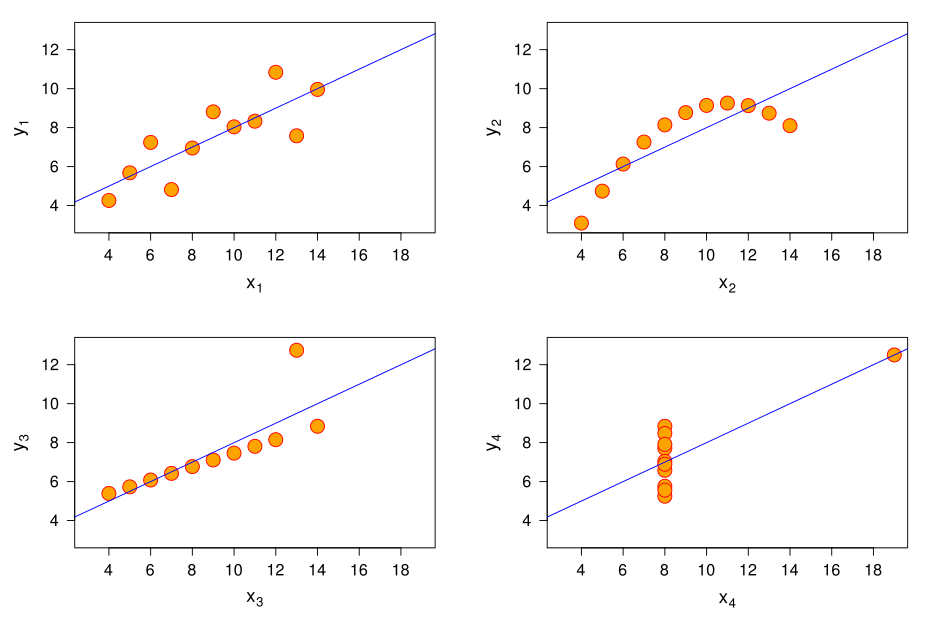
\includegraphics[scale=0.5]{expressed/Anscombe.png}\centering
      \caption[Anscombe quartet --- why data should always visualy checked]
      {\label{fig:Anscombe}\textbf{Anscombe quartet --- why data should always
      visually checked.}\smallbreak{} All the datasets displayed here have equal
      or very similar descriptive statistic indicators.}
\end{figure}

\section{Expressed or not expressed}
\label{sec:ExpressedOrNot}

While it can seem as a trivial concept and might be overlook, whether a specific
molecule is expressed --- or not --- in a given condition, can actually have
an extensive impact on the results of the analyses, particularly when integrating
proteome and transcriptome together.

For example, the Pearson correlation coefficient is very
sensitive to outliers and null values. If for both samples, a vast number of
null values are recorded, this will lead to a greater similarity.
Hence, it is important that the data used for the analysis is meaningful in
its whole, i.e.\ a null value has still to be an observation and translates
a lack of expression (and not a lack of observation).

\begin{figure}[!htbp]
    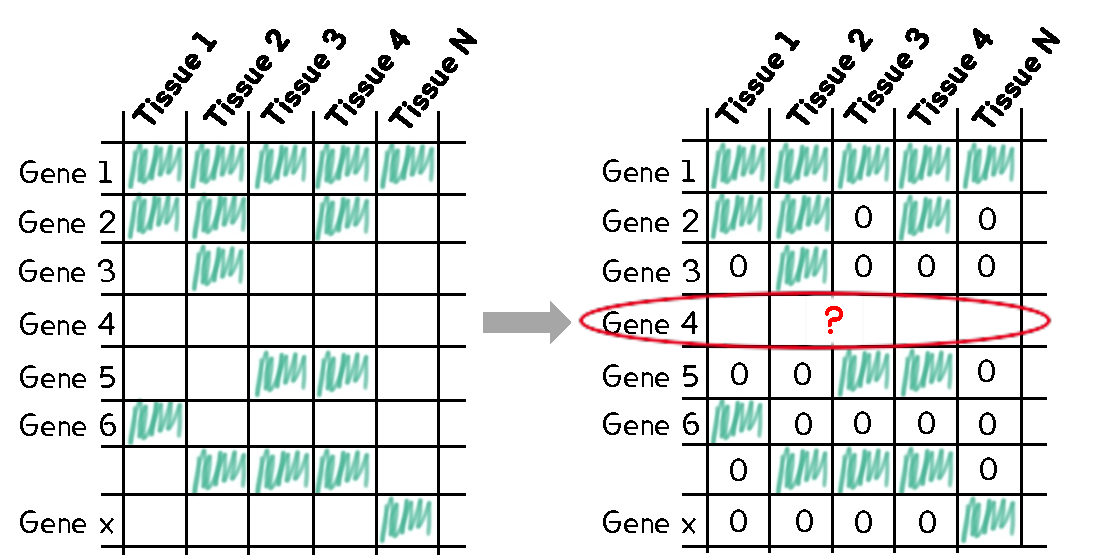
\includegraphics[scale=0.7]{expressed/expressedNotExp.pdf}\centering
      \caption[Expressed or not: several cases illustrated]
      {\label{fig:DefineExpression}\textbf{Expressed or not: several cases
      illustrated.}\smallbreak{} Genes as \emph{gene 1} are unequivocal: they have been
      detected in all the different tissues. Genes that have been quantified in
      \emph{some} of the conditions are, in principal, detectable with the
      protocol of sampling and quantification used for the assay.
      For these genes, when no signal is collected, I assume this is a true $0$.
      The genes without any quantification
      in any tissue, e.g.\ gene 4, are discarded from the remaining analysis as
      I can't state
      either there are truly absent from the biological sample or it has to due
      to the protocol at use; they are \emph{undefined}. The same approach is used
      for the transcriptome and the proteome.}
\end{figure}

\subsection{The undefined}%\KOMAoptions{parskip=false}
\label{subsec:ExpressedOrNot-undefined}
If a protein or transcript is never found in any of the samples of a dataset,
then I considered that we can not determine if the protein or transcript was
either truly not expressed or, for any reason, was not capture while the library
preparation or the identification/quantification steps. Hence, those are
excluded from the analyses as I can not resolve precisely if this is a
technical artefact or a biological truth. This case is illustrate by the row
circled in red in~\cref{fig:DefineExpression}.

\subsection{Expression in a dataset}
\label{subsec:ExpressedOrNot--expDataset}
By contrast, if a protein or a transcript is expressed in some samples of the
dataset, then, whenever no expression was recorded in the other
samples, I consider that the expression of the considered macromolecule is truly
null for those samples.

\subsection{Expression within a sample}
Due to the technical (and biological) differences between proteomics and
transcriptomics, I use different thresholds to define the expression of a protein
or a transcript.

\subsubsection{Expressed protein}
On the proteomic side, I consider that a protein is expressed if it has been
identified and quantified. In other words, if the expression value of a protein
is greater than zero in a sample, I consider it as expressed.

\subsubsection{Expressed transcript}\KOMAoptions{parskip=half*}\label{subsubsec:exprTrans}
It is a bit more complex on the transcriptomic side as we have to account for
technical noise, but we can also expect ``translational noise'' \citep{rnaseq-2009},
\citep{lowNoiseLimit}.
While we can empirically evaluate it for each \Rnaseq\ dataset \citep{ramskoldan:2009},
there is a widespread threshold used in the literature:
1 \gls{FPKM} (or \gls{RPKM}).

I have used this threshold to run (at least once) all the analyses since
many datasets are enriched for \mRNAs. Moreover, the \Cref{ch:Integration}
focus is the comparison of proteomic and
transcriptomic data. In fact,~\citet{Hebenstreit:2011} showed in their study
\paper{\citetitle{Hebenstreit:2011}}, that to be translated into a protein,
a \mRNA\ should present an expression at least equals to 1 \gls{RPKM}.

As our current study focuses on the comparison of proteomic and transcriptomic
data, all the analyses have been run with this threshold. It is worth mentioning
that parts of the analyses have also been done either without
any threshold (i.e.\ the same definition used with the proteins has been applied)
or with a threshold of $5$ \glspl{FPKM}.

\subsection{Limitation of the study}
While I have compared the list of undefined, expressed and unexpressed molecules
the bulk of the analysis has been done on the common ones.

In other words, if a \mRNA\ --- or protein --- is not expressed in at least
one sample in \emph{every and each} of the datasets used for the analysis,
it will be excluded from the main part of it.



